\chapter{Visualisation expérimental d'un mode localisé}
Différents problèmes rendent la mesure d'un mode localisé difficile.

Tout d'abord il n'est pas trivial de trouver une configuration qui permette la génération d'un mode localisé car c'est un phénomène difficile à visualiser et ce même en simulation. La fréquence de résonance du défaut doit se trouver sur le bords d'une bande interdite (à l'intérieur) afin de pouvoir la visualiser sur les coefficients de transmission et réflexion. En effet, la propagation de l'onde dans le réseau est difficile: la bande interdite rend la décroissance de l'onde exponentielle. Par conséquence, exciter le mode de défaut est difficile et même s'il est excité la pression reste localisé. Celle-ci n'est alors pas visible sur les coefficients de transmission et de réflexions qui sont issues de mesures à l'entrée et la sortie du réseau sauf dans le cas d'un réseau constitué de peu d’éléments et avec un défaut en bord de bande.


\subsection{Protocole expérimental}
Le banc de mesure utilisé est constitué d'un tuyau de 60 trous sur lequel peuvent être fixé des résonateurs variablesb (les dimensions sont présents en annexe) ou bien des bouchons. La source utilisée est celle du capteur d'impédance: celui-ci est fixé à une des extrémités du réseau et est relié à une carte d'acquisition piloté par le logiciel spécialisé du CTTM. Ce capteur dispose de 2 microphones et permet donc de calculer directement le coefficient de réflexion du réseau. Afin de pouvoir calculer le coefficient de transmission, un autre microphone est ajouté $10~cm$ après le dernier résonateur.
\todo{citer une annexe sur la démo du coefficient de transmission et mettre la bonne annexe sur les dims des resonateurs}

\bigskip

A l'autre extrémité du réseau se trouve une embouchure de sortie anéchoïque préalablement réglée afin que le coefficient de réflexion au bout du réseau soit le plus faible possible.
\todo{une annexe sur la source anéchoi => explication sur le reglage+figure?}


\section{Mesure du coefficient de réflexion et de transmission du réseau}
On s'intéresse tout d'abord à la mesure du coefficient de réflexion et de transmission dans le réseau. Bien qu'un mode localisé soit dure à observer dans ces conditions, le but est de chercher la fréquence précise à la quelle celui-ci à lieu afin de pouvoir par la suite mesure ce mode à l'intérieur du réseau. Pour cela on ne prend que 5 résonateurs (avec un défaut sur le troisième) afin que le mode localisé puisse "déborder" sur les bords du réseau et ainsi qu'il soit mesurable (dans cette configuration l'atténuation lié au bandes interdites est moins importante). Les résonateurs ont une longueurs de cavité de $16~cm$ et le défaut de $8~cm$. Les courbes figure ~\ref{ref1} et ~\ref{trans1} correspondent aux coefficients de réflexion et de transmission pour cette configuration.

\begin{figure}[!h]
\centering
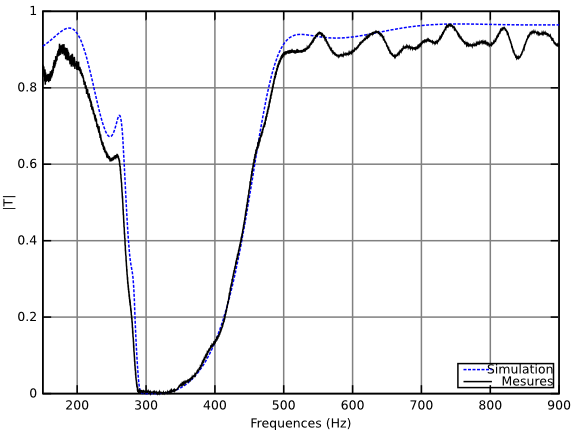
\includegraphics[scale=0.4]{images_chp3/5HR165_nodefect.png}\hfill
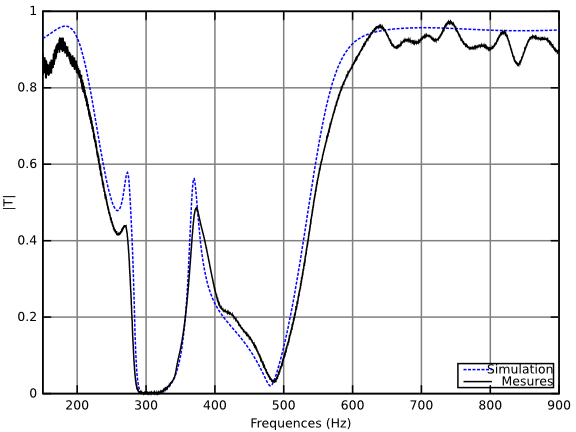
\includegraphics[scale=0.4]{images_chp3/5HR165_8cm_pos3.png}
\caption{\label{ref_trans1} Coefficient de transmission du réseau dans un cas sans défaut et avec défaut. Les courbes de simulations et de l’expérience sont superposées.}
\end{figure}

On constate qu'un pic de transmission est visible dans la bande interdite tant théoriquement qu'expérimentalement: le défaut permet à l'onde de traverser le réseau pour une fréquence donnée alors que dans le cas ou celui-ci n'est pas présent aucune transmission n'est possible. Ce comportement laisse supposer qu'un mode localisé est présent au niveau du défaut: si on augmente le nombre de résonateur, l'atténuation est plus forte et le pic disparaît, le mode est alors complètement localisé.

Ces résultats se retrouvent aussi sur la réflexion.
%
%\begin{figure}
%\centering
%\includegraphics[scale=0.3]{•}\hfill
%\includegraphics[scale=0.3]{•}
%\caption{\label{ref_trans1} Coefficient de transmission du réseau dans un cas sans défaut et avec défaut. Les courbes de simulations et de l'expériences sont superposées.}
%\end{figure}
\todo{coefficient de réflexion  pour ce truc la}

\section{Mesure d'un mode localisé par insertion de capteur dans le réseau}
Une fois la fréquence du mode de défaut relevée sur les coefficients de réflexions et transmissions on augmente le nombre de résonateurs de part et d'autre du défaut afin de créer un mode complètement localisé. Afin de pouvoir quand même exciter le mode localisé, une source est placé dans un des orifices au voisinage du défaut. Un microphone est inséré dans le réseau afin de mesure la pression en n'importe quel point. La pression RMS mesurée dans le tube est représenté figure ~\ref{p_tube} pour une configuration avec et sans défaut.

\begin{figure}[!h]
\centering
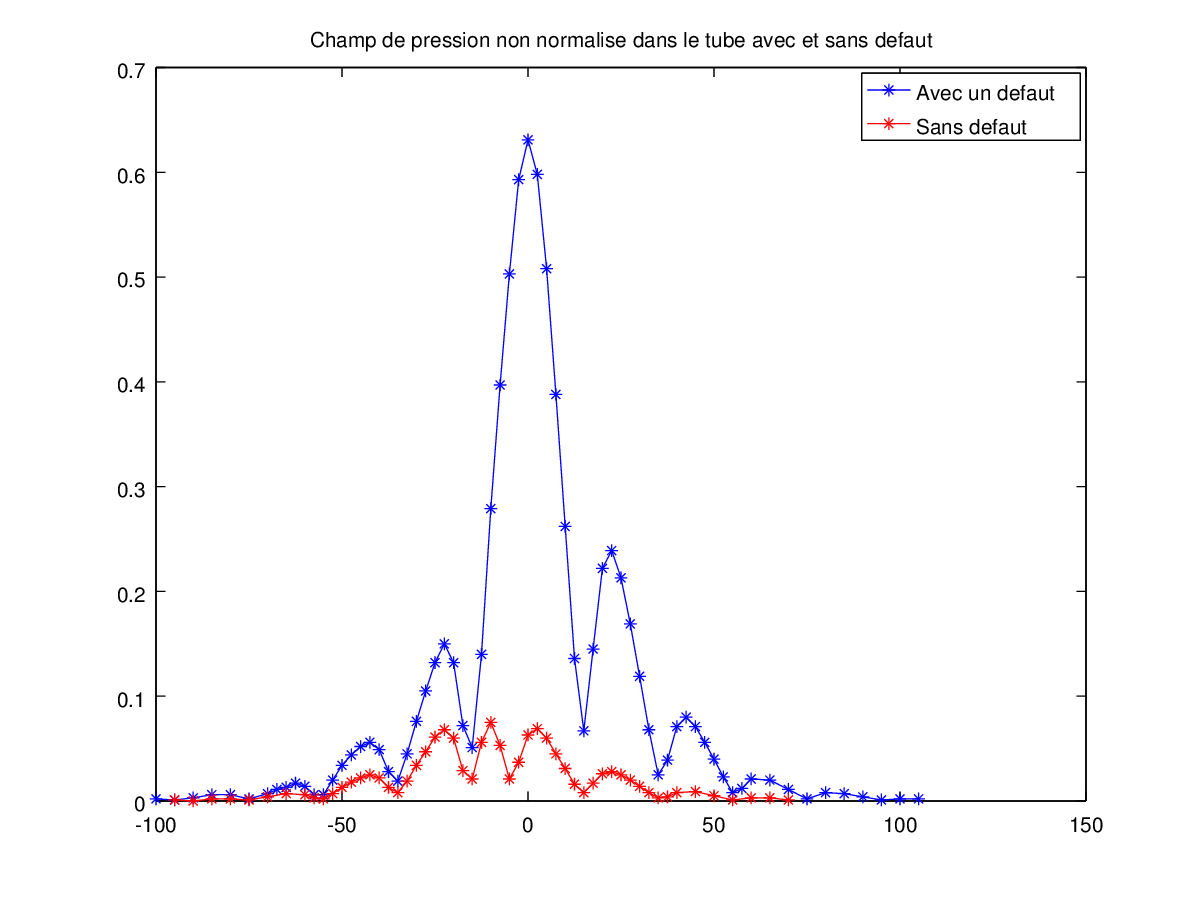
\includegraphics[scale=0.5]{./images_chp3/non_norm_lin.png}
\caption{\label{_tube} Pression RMS mesurée dans le réseau afin de mettre en évidence un mode localisé.}
\end{figure}

On constate que les niveaux de pression mesurés sont près de 10 fois plus élevé dans le cas ou un défaut est présent. De plus, la décroissance à mesure qu'on s'éloigne du défaut est très importante: on est donc bien en présence d'un mode localisé. Il est a noté que dans cette configuration le niveau maximum dans le réseau ne ce situe pas au niveau de la source mais du défaut (ce qui n'est pas le cas quand il n'y a pas de défaut).
